\chapter{Architecture}
\label{ch:architecture}

\begin{quotation}
“The greatest pleasure in life is doing what people say you cannot do.”
{\small\it -- Walter Bagehot (British political Analyst, Economist and Editor, one of the most influential journalists of the mid-Victorian period.1826-1877) }
\end{quotation}

In this section we explain the overall architecture of the system and our the proposal for the problem presented in distributed data stores with flexible rather and stringent consistency requirements. First of, we have a general overview of the proposal in section~\ref{architecture:overview}. The following sections deal with the design decisions made and the motivation behind them. For that, we aim at explaining them in as much detail as possible for the sake of comprehension of the following chapter, Implementation. Each of the steps in the design process is justified, and in particular those related to asynchronous replication using RPC mechanism for the architectural changes introduced into HBase with the QoD module. We do that while taking into account what are the main requirements to fulfill our goals as specified in section~\ref{architecture:requirements}. Therefore, we are able to show the reasoning behind the main architectural design decisions and showcase the main goal scenario as in a "thousand feet" high-level view of the system first of all~\ref{fig-high-level}, and secondly in a more detailed manner in section~\ref{architecture:extensions}. Following and up to the evaluation, we delve into the proposed changes in order to verify the feasibility of the implementation as well as what scenarios are best suited to our definition of consistency.

\section{System overview}\label{architecture:overview}
% How the containers replicate thigns with the QoD
A three-dimensional vector constraint model based on~\cite{Santos:2010} is implemented in the form of the corresponding QoD paradigm, shipping updates for replication, or retaining them for later shipment as mentioned. For that to be possible, we have used a set of customized data structures, which hold the values of the database rows we desire to check according to some specific field we might be interested in (e.g column family) for replication. 

To compare and track the QoD fields, that act as constraints to replicate updates, against these stored entries, we defined data \emph{containers} which are useful to keep track of the current value of the vector-field selected to bound replication to, and secondly the maximum value it will be allowed to reach before updates are flushed to the slave cluster and then reset again. That is as what we call the QoD percentage of updates replicated (according to the selected vector-field bound, e.g $\sigma$). The process is partly automated, of by now, we just define it at run-time (or by the developer later) by adding a parameter into the HBase console to define a vector-field specific bound.

\section{From eventual consistency to vector-field bounded consistency}\label{architecture:requirements}
This section explains and drives the motivations in the following steps of the chapter in order to justify how and why we made those during the implementation process later of the architecture of our replication module into HBase.

\subsection{Replicated Storage}
Regarding replicated Storage we have the following requirements: 

\begin{enumerate}
\item Separate concerns in terms of data semantics and replication.
\item Replication is still asynchronous but with a higher degree of consistency guarantees, based on a vector-field consistency model that allows defining the constraints and limits for each type of data then.
\item Partitioning is allowed but eventual consistency allows to reconcile changes autonomously, while grouping of operations enforce maintaining atomically replicated updates so avoiding the first in case of long periods of disconnection to the network (it is already possible to define a rety timeout in HBase in case of partitioning so we do not need to focus on that but rather on the grouping part)
\end{enumerate}

Given the fact that HBase already provides an eventual consistency mechanisms through Remote Procedure Calls in order to replicate items, we chose that data store as the default system to first implement our proposed architecture. Also, we can enhance the current multi-row atomic model, using an approach that can also relate column families between updates in order to provide the same atomicity at the column-level. That is potentially useful for distinguishing updates between cluster update owners and users or applications that need those updates from another cluster for the fact of being consistently up to date in regards to their own local data center ongoing update operations. The overall architecture layout is presented in Figure~\ref{fig-high-level} with this idea in mind showing the main goal scenario for it in Figure ~\ref{fig-high-level}. A simple interface introducing a vector-field consistency model is later shown with the implementation of this architecture details.

\begin{figure}[t]
\centering
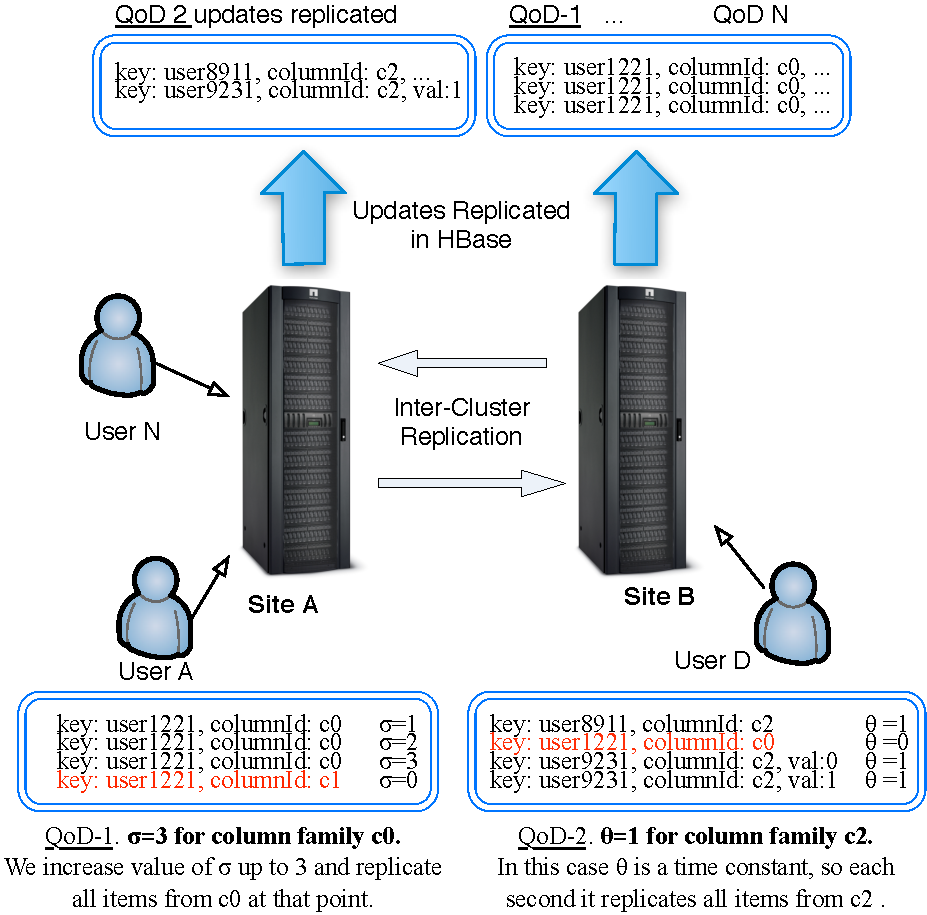
\includegraphics[width=0.8\linewidth]{figs/highlevel.pdf}
\caption{HBase QoD high-level}
\label{fig-high-level}
\end{figure}

\subsection{Remote Procedure Calls}
HBase implements remote procedure calls for the replication of items between servers or clusters. These mechanisms have been proven a useful paradigm for providing communication across a network~\cite{Birrell:1984}. An RPC mechanism is mainly responsible for providing control of data transfer between a source and a destination location, called \emph{ReplicationSource.java} and \emph{ReplicationSink.java} respectively in HBase. Having discussed that in depth with contributors of the HBase community is clear how this operates in HBase. The ReplicationSource tails the WAL and then sends the WALEdit to the ReplicationSink via RPC. In other words, the code applies the edits to the slave cluster via a remote call to the method in the RPC sink (calling a method named ReplicateLogEntries remotely).


\section{Technologies used and development method}\label{method}
In order to introduce a new HBase-QoD module into the previous architecture, we have first studied the system to get familiar with it and identify the best locations for new code added. Therefore we take into account the original programmed inner-workings of the data store logical flow and that ensures correctness and validity of the paradigm implemented later in next chapter. 

\begin{enumerate}
\item First identifying the source and destination of updates.
\item Secondly, defining a QoD vector-model based on the schema design of HBase so we can reach our goals.
\item Finally integrating both parts into the same system, and providing a mechanism to switch on and off the module at run time into HBase.
\end{enumerate}

% Implementation details, such as WALEdit, algorithm, images of QoD inside DC, etc. 
HBase is written in Java and its replication mechanisms are related to a Write Ahead Log (WAL) that also ensures durability of updates and disaster recovery. Replication must be enabled for shipping updates between peer cluster locations in remote or nearby data centers. The process of replication is carried out asynchronously so there is not additional overhead or latency introduced in the the master server during that operation.  Although, since the process is not strongly consistent, in write heavy applications an slave can have stale data in the order of more than just a few seconds according to the eventual consistency approach. Therefore, until the last update first commits to the local disk, it cannot be seen replicated in a remote location. To keep control of staleness, we plug a QoD module called HBase-QoD which provides and takes advantage of a sorted priority queue of update items filtered and scheduled for replication accordingly. Thereafter, when the method completes, updates are shipped in an ordered fashion by enforcing currently defined QoD bound constraints over data marked for delivery to a remote cluster location. For write intensive applications that can be both beneficial in terms of peaks of bandwidth usage and also reduced staleness of data we believe.


Using the QoD involves a temporal caching of updates until the threshold set in the three-dimensional vector is reached, so having a caching mechanism that stores those edits for further evaluation against constraints (namely time, sequence and value) We can then decide if an item or group of items is due to propagation for replication or not.

\section{Extensions to HBase internal mechanisms}\label{architecture:extensions}
The section focuses on the reasoning behind the internal changes to the HBase mechanisms proposed to include into the system in order to rule updates selectively during replication.

We extend HBase, adding updates due to be replicated in a priority queue according to their own QoD in each case. Thereafter once the specified QoD threshold is reached another thread from HBase in the form of Remote Procedure Call collects and ships all of them at once.

\begin{figure}[t]
\centering
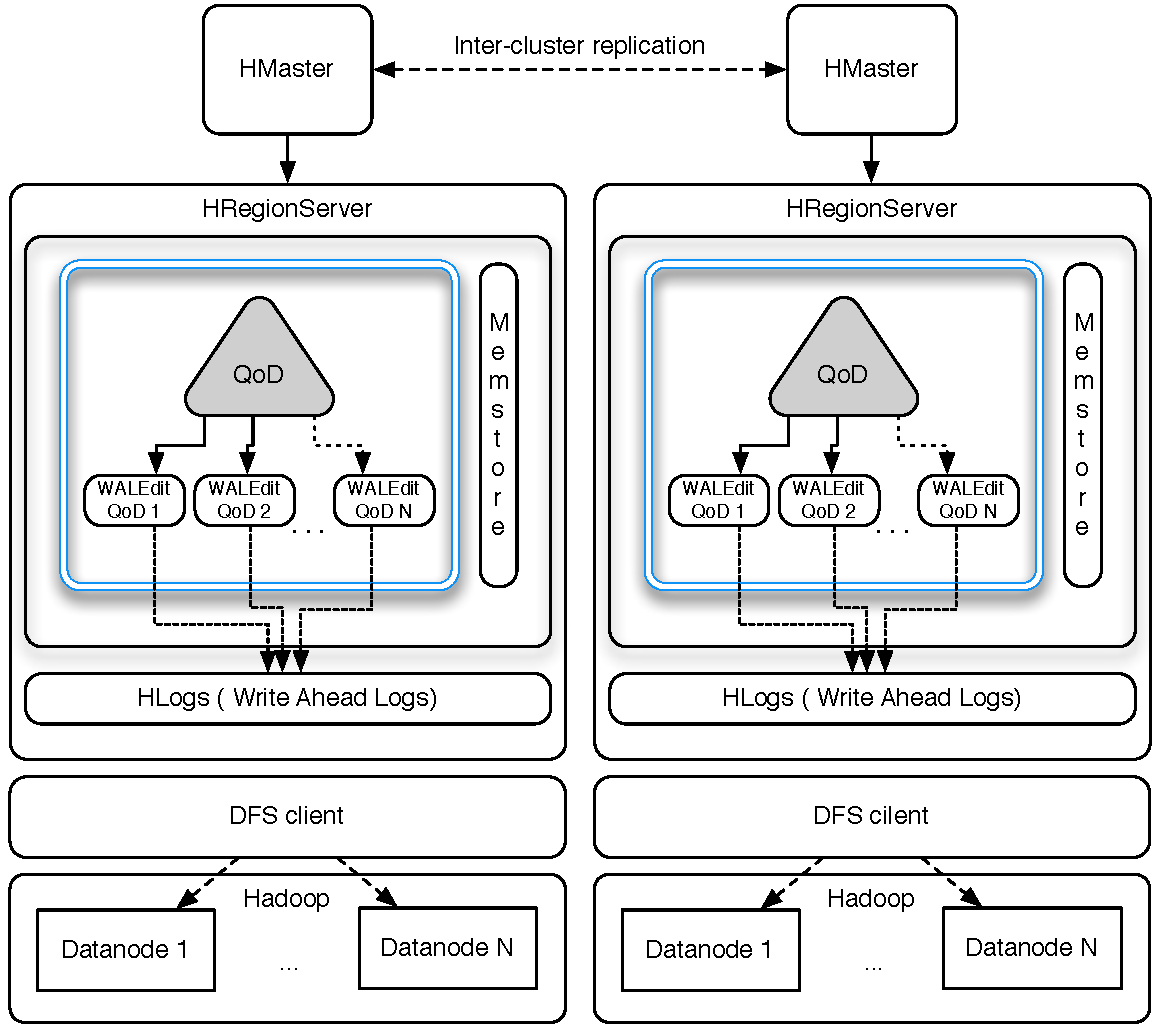
\includegraphics[width=0.8\linewidth]{figs/multi-site.pdf}
\caption{HBase QoD operation}
\label{fig-qod-module}
\end{figure}

In Figure~\ref{fig-qod-module} we can briefly observe how the QoD module plugs into HBase, intercepting the incoming updates from the upper layers and passing them down and the resulting outcome to the Write Ahead Logs for later replication.

\emph{ReplicationSource.java} is a key part of HBase in these regards and it is unveiled after researching the code that is the right location to modify the logic of the shipment of edits to control those according to a defined HBase-QoD. For that purpose we design a custom data structure in HBase reusing the existing classes WALEdits (from HBase), ConcurrentHashMap (a Java library) so we are able to set up the storage locations for the updates and identify them according to a container identifier. Later, there we apply each given QoD (e.g. tablename:columnFamily) and the actual value of the vector while we check for the condition that triggers replication once it matches or surpasses the given bound in the container id. As soon as we have some incoming input from clients we process the updates feeding the QoD.

\section{Typically distributed and replicated deployment}\label{distributed-architecture}
In distributed clusters Facebook is currently using HBase to manage the messaging information across data centers. That is because of the simplicity of its consistency model, as well as the ability of HBase to handle both a short set of volatile data and ever-growing data, that rarely gets accessed more than once. More specifically, in their architecture reports, a Key for each element is the userID as RowKey, word as Colum and messageID as Version and finally the value like offset of word in message (Data is sorted as: \emph{userId, word, messageID}). That implicitly means that searching for the top messageIDs of a specific user and word is easily supported, and therefore queries run faster in the backend.

%%In this work we assume the need for having a tailored replication mechanism that targets applications which require finer levels of consistency, others have previously used Snapshot Isolation techniques or as COPS the ALPS properties. In a previous paper, a.k.a as the conit consistency model from Duke University \cite{Duke:2001}, the system is mainly focused on generality not practicality. We prefer the later because we find it more rewarding to users that need to integrate a fully functional system with a replication framework that bests optimizes geo-replication costs. Actually there is an opened issue on the HBase community site for this particular matter \cite{JIRA-1}. In distributed clusters Facebook is currently using HBase to manage the messaging information across data centers not Cassandra~\cite{FacebookHBase}, that is because of the simplicity of consistency model as well as the ability of HBase to handle both a short set of volatile data and an ever-growing data set that rarely gets accessed more than once. More specifically, in their architecutre reports, a Key for each element is the userID as RowKey, word as Colum and messageID as Version and finally the value like offset of word in message (Data is sorted as: <userId, word, messageID>). That implicitly means that searching for the top messageIDs of an specific user and word is easily supported, and therefore queries can run faster in the backend.
%So, for filtering purposes, with our new proposal and implementation, that could directly enable administrators of the clusters to create quality-of-data policies that can analyze fetched data  isrt by inspecting some given bounds or semantics, and then receiving them on the master server at the other end of the replication chain if a match occurs. At first, we will be enhancing the eventual consistency model for inter-site replication in HBase by using an adaptive consistency model based on Service Level Objectives agreed or defined. The idea can be somehow similar to the "pluggable replication framework" proposed within the HBase community [ref here], so our work is two-fold purpose. First contributing to the open source community of HBase but also extending it with some extra capabilities, for that later we will implement batching of updates within our QoD framework.

With the eventual consistency enforcement provided, updates and insertions are propagated asynchronously between clusters so Zookeeper is used for storing their positions in log files that hold the next log entry to be shipped in HBase. To ensure cyclic replication (master to master) and prevent from copying same data back to the source, a sink location with remote procedure calls invoked is already into place with HBase. Therefore if we can control the edits to be shipped, we can also decide what is replicated, when or in other words, how soon or often.

%% Build up here on WAL, ReplicationSource, etc. Also high-level architecture drawings,
In order to provide bounded consistency guarantees with QoD, we add it to the inner workings of HBase. There are existing command line tools as CopyTable in HBase where one can manually define what is going to be replayed to the log and this is useful for cases where new replicas need to be put up to date or in disaster recovery too. In particular, we focus our implementation efforts into organizing a list of items in memory (extending the original structure reflected for the updates to be shipped), where we can apply our QoD principles and directly enforce constraints. We do that by defining our bounded divergence model over data which is indexed and queried by key (containerId), and can be enforced through time constraints (T), sequence (number of pending updates) and value (percentage of changes).